\documentclass[12pt,handout]{beamer}

%\documentclass{beamer}
\usetheme{Boadilla}
\useoutertheme{split}

\usepackage{amsmath}
\usepackage{fancyvrb}
\usepackage{tikz}
\usetikzlibrary{shapes, calc, shapes, arrows, graphs}

\usepackage{amsmath,amssymb}

\usepackage{xcolor}

\definecolor{xvectorcolor}{HTML}{77933C}
\definecolor{exerciseblue}{RGB}{200, 200, 247}

\titlegraphic{
\includegraphics[scale=0.1]{abremodlogo.png}}

\title{Gurobi Training}
\author{Abr\'emod}

\begin{document}


\begin{frame}
\frametitle{Column Generation}
\begin{itemize}
  \item Give Gurobi a small portion of the variables
    \begin{itemize}
      \item Variables left out of model are effectively fixed to 0
    \end{itemize}
  \item Iteratively add additional columns
    \begin{itemize}
    \item Solve LP with a subset of all possible variables
    \item Identify and add variables that would improve the solution
    \end{itemize}      
    \item More columns than rows
    \begin{itemize}
      \item Low proportion of variables have nonzero values
      \item Number of potential variables may even be exponential
      \item Ratio of rows to columns should be close to 0
    \end{itemize}
\end{itemize}
\end{frame}

\begin{frame}
\frametitle{Column Generation Theory}
\begin{eqnarray}
z^* = \min_x && \sum_{i \in I} c_i x_i  \nonumber \\
\mbox{s.t.} && \sum_{i \in I} a_{ij} x_i  = b_j : \pi_j,\;\;j \in J \nonumber \\
&& x_i \ge 0,\;\;i \in I. \nonumber
\end{eqnarray}

\begin{itemize}
\item The reduced cost of variable $i$ can be computed as: $c_i - \sum_{j} a_{ij} \pi_j$
\item If $c_i - \sum_{j} a_{ij} \pi_j \ge 0$ for all $i \in I$, we have a proof of optimality.
\item Can compute the reduced cost even for variables not yet added to the model.
\end{itemize}
\end{frame}

\begin{frame}
\frametitle {What you need to know}
\begin{itemize}
\item Models can be solved iteratively
	\begin{itemize}
	\item Model remains in memory after a call to Model.optimize().
	\item Can then call addVar to add new decision variables, then re-optimize.
	\end{itemize}
\item Variables are added after constraints are added.
     \begin{itemize}
     \item Pass a Column object in to Model.addVar to back-populate constraints.
     \end{itemize}
\item Compute reduced costs from dual prices.
     \begin{itemize}
     \item Choose variable(s) with negative reduced costs to add to the model.
     \item If all reduced costs are non-negative, then the existing variables produced an optimal solution.
     \end{itemize}
\end{itemize}
\end{frame}

\begin{frame}
\frametitle {Columnwise modeling in Gurobi}
\begin{itemize}
  \item Rowwise Pattern
  \begin{itemize}
    \item Create variables (columns)
    \item Create LinExpr list of (coef, Var) pairs
    \item Create constraints (rows) in terms of LinExpr
  \end{itemize}
  \item Columnwise Pattern
  \begin{itemize}
    \item Create constraints (rows)
    \item Create Column list of (coef, GRBConstr) pairs
    \item Create variables in terms of Column
  \end{itemize}
\end{itemize}
\end{frame}


\begin{frame}
\frametitle{Gurobi API for column generation}
\begin{itemize}
\item Model.addVar(lb, ub, obj, vtype, name, column)
\item Column(coeffs, constrs)
     \begin{itemize}
     \item col = Column(3, c1)
     \item col = Column([1, 2], [c1, c2])
     \end{itemize}
\item Dual values come from Pi attribute of Constr objects.
\end{itemize}
\end{frame}

\begin{frame}[containsverbatim]
\frametitle{Transportation Problem}
\begin{eqnarray}
\min_{x} && \sum_{i \in I} \sum_{j \in J} c_{ij} x_{ij} \;\; \mbox{(minimize shipping costs)} \nonumber \\
\mbox{s.t.} && \sum_{i \in I} x_{ij} = d_j,\;\;j \in J \;\; \mbox{(satisfy demand)}\nonumber \\
&& \sum_{j \in J} x_{ij} \le u_i,\;\;i \in I \;\; \mbox{(don't exceed capacity)} \nonumber \\
&& x_{ij} \ge 0, \;\;i \in I,\;j \in J \;\; \mbox{(ship nonnegative quantities)} \nonumber
\end{eqnarray}

Consider $x_{ij}$ for a particular warehouse $i$ and customer $j$.

{\scriptsize
\begin{verbatim} 
col = Column([1, 1], [capacity_constrs[i], demand_constrs[j]])
var = model.addVar(obj=ship_costs[i][j], column=col)
\end{verbatim}
}
\end{frame}

{
\setbeamercolor{background canvas}{bg=exerciseblue}
\begin{frame}
  \frametitle{Exercise}
  \begin{itemize}
    \item Write addColumn method in FacilityLocationColumn.
    \item Problem should solve exactly like the row-oriented model
  \end{itemize}
\end{frame}
}

\begin{frame}
  \frametitle{Column Generation Loop}
  \begin{itemize}
  \item Can add any columns with negative reduced costs
  \item Need to add at least one column per iteration
    \begin{itemize}
    \item Add columns with negative reduced costs
    \item Can add multiple columns per iteration to reduce number of iterations
    \end{itemize}
  \end{itemize}
\end{frame}

{
\setbeamercolor{background canvas}{bg=exerciseblue}
\begin{frame}
  \frametitle{Exercise}
  \begin{itemize}
    \item Write getRC(warehouse, customer) method
    \item Write addColumns() method
    \item Experiment with different strategies
      \begin{itemize}
        \item Add first variable with negative reduced cost
        \item Add all variables with negative reduced costs
        \item Add variable with most negative reduced cost
      \end{itemize}
  \end{itemize}
\end{frame}
}


\begin{frame}
\frametitle{What is a Convex Program?}
\begin{block}<+->{Definition}
\begin{eqnarray}
\mbox{minimize:} && f(x_1, x_2, \ldots, x_n) \nonumber \\
\mbox{subject to:} && g_i(x_1, x_2, \ldots, x_n) \le b_i, \;\; i = 1, \ldots, m \nonumber \\
&& x_j \ge 0,\;\;j = 1, \ldots, n \nonumber
\end{eqnarray}
f, $g_i$ are all convex.
\end{block}
\end{frame}

\begin{frame}
  \frametitle{Convexity}
  \begin{itemize}
    \item Averages are better than extremes.
    \item If $x$ and $y$ are feasible, then $\frac{x + y}{2}$ is feasible.
    \item The objective function evaluated at $\frac{x + y}{2}$ must be better than the average of $x$ and $y$. \\
\item All local optimum are globally optimal
  \end{itemize}
\end{frame}


\begin{frame}
\frametitle{What does convex look like?}
\begin{itemize}
\item Slopes are non-decreasing as we move from left to right.
\item Not as obvious in multiple dimensions.
\end{itemize}
\begin{tabular}{lc}
Convex &
\begin{tikzpicture}
\draw (0,0) to [out=-90,in=-90] (2,0);
\end{tikzpicture} \\
Concave &
\begin{tikzpicture}
\draw (0,0) to [out=90,in=90] (2,0);
\end{tikzpicture} \\
Both &
\begin{tikzpicture}
\draw (0,0) to (2,1);
\end{tikzpicture} \\

Neither &
\begin{tikzpicture}
\draw (0,0) to [out=0,in=180] (2,1); 
\end{tikzpicture} \\
\end{tabular}

\end{frame}

\begin{frame}
\frametitle{Convex Quadratic Programming}
\begin{align*}
\mbox{minimize:} & \sum_i c_i x_i + \sum_{i,j} q_{ij} x_i x_j \nonumber \\
\mbox{subject to:} & \sum_i a_{ik} x_i + \sum_{i,j} d_{ijk} x_i x_j  \le b_k
\end{align*}
\begin{itemize}
\item All functions must be convex (for minimization, $\le$ constraints).
\item Unlike in the linear case, minimize/maximize; $\le$, $\ge$ are not interchangeable.
\end{itemize}
\end{frame}

\begin{frame}
\frametitle{Feasible Region}
\begin{tabular}{ccc}
Linear & \hspace{1in} & Quadratic \\

\begin{tikzpicture}
\draw [fill = blue] (0,0) to (1,1) to (1,2) to (0,1) to (0,0);
\end{tikzpicture}  &  &

\begin{tikzpicture}
\draw [blue, fill = blue] (0,0) to (1,1) to (1,2) to (0,1)  ;
\draw [blue, fill = blue] (0,0) [out=0, in = 270] to (1,1);
\draw [blue, fill = blue] (0,1) [out=75, in = 200] to (1,2);
\end{tikzpicture} \\
\end{tabular}
\end{frame}


\begin{frame}
\frametitle{What you can't do with Quadratic Expressions}
\begin{itemize}
  \item nonlinear equality constraints
  \item $x_i (1-x_i) \le 0$ to simulate binary variables.
  \item ``Bilinear'' programming $(\sum_i x_i \cdot y_i)$.
    \begin{itemize}
      \item pricing and allocations (price and sales variables)
      \item blending problems (concentrations and quantities)
    \end{itemize}
\end{itemize}
\end{frame}

\begin{frame}
\frametitle{What is allowed}
\begin{itemize}
  \item $x^tQx$ Hessian Matrix $Q$ must be positive definite.
    \begin{itemize}
      \item All eigenvalues are positive.
    \end{itemize}
  \item $f(\alpha x + (1-\alpha) y) \le \alpha f( x ) + (1-\alpha) f(y)$
  \item Maximizing a concave function
  \item lower bound on concave function ($f(x) \ge b$ for concave $f$).
\end{itemize}
\end{frame}

\begin{frame}
  \frametitle{Convexity}
  \begin{itemize}
    \item $f(x)$ convex $\equiv -f(x)$ concave
    \item if $f(x)$ and $-f(x)$ are both convex then $f(x)$ is linear
      \begin{itemize}
        \item $f(x) = b \equiv f(x) \le b \mbox{\ \bf and } f(x) \ge b$
        \item only linear equality constraints are allowed
      \end{itemize}
    \item Hard to verify in general
      \begin{itemize}
        \item Harder than actually optimizing
        \item Your responsibility to give Gurobi convex problems
        \item Gurobi ErrorCodes if it discovers non-convexity
          \begin{itemize}
            \item QCP\_EQUALITY\_CONSTRAINT
            \item Q\_NOT\_PSD
          \end{itemize}
      \end{itemize}
  \end{itemize}
\end{frame}

\begin{frame}
\frametitle{Building a Quadratic Model with Gurobi}
\begin{itemize}
\item GRBQuadExpr
\begin{itemize}
\item GRBQuadExpr.addTerm(coef, var1, var2)
\end{itemize}

\begin{itemize}
\item GRBQuadExpr.addTerm(coef, var)
\end{itemize}
\end{itemize}
\end{frame}

\begin{frame}
\frametitle{Example: Linear Regression}
\begin{itemize}
  \item Input: (x, y) pairs
  \item Regression Model: $y_i = \mbox{slope} \cdot x_i + \mbox{intercept} + \mbox{residual}_i$
  \item Minimize: $\sum_i \mbox{residual}^2_i$
\end{itemize}
\end{frame}

\begin{frame}
\frametitle{Example: Sample Data}
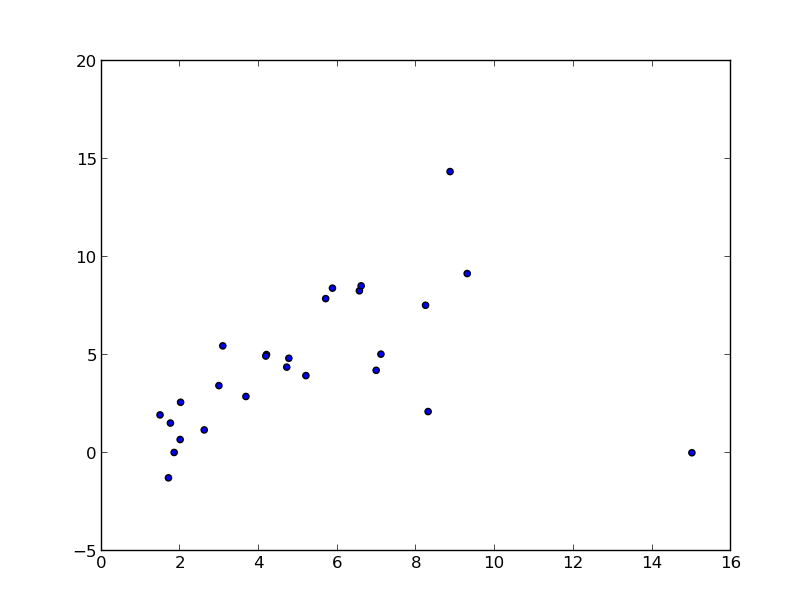
\includegraphics[scale=0.5]{regression.png}
\end{frame}

{
\setbeamercolor{background canvas}{bg=exerciseblue}
\begin{frame}
  \frametitle{Exercise}
  \begin{itemize}
  \item Solve regression as a QP
  \item Compare results with Minimize: $|\sum_i \mbox{residual}_i|$
  \end{itemize}
\end{frame}
}

\end{document}
